\documentclass[a4paper]{article}
\usepackage[pdftex]{hyperref}
\usepackage[latin1]{inputenc}
\usepackage[english]{babel}
\usepackage{a4wide}
\usepackage{amsmath}
\usepackage{amssymb}
\usepackage{algorithmic}
\usepackage{algorithm}
\usepackage{ifthen}
\usepackage{listings}
% move the asterisk at the right position
\lstset{basicstyle=\ttfamily,tabsize=4,literate={*}{${}^*{}$}1}
%\lstset{language=C,basicstyle=\ttfamily}
\usepackage{moreverb}
\usepackage{palatino}
\usepackage{multicol}
\usepackage{tabularx}
\usepackage{comment}
\usepackage{verbatim}
\usepackage{color}

%% pdflatex?
\newif\ifpdf
\ifx\pdfoutput\undefined
\pdffalse % we are not running PDFLaTeX
\else
\pdfoutput=1 % we are running PDFLaTeX
\pdftrue
\fi
\ifpdf
\usepackage[pdftex]{graphicx}
\else
\usepackage{graphicx}
\fi
\ifpdf
\DeclareGraphicsExtensions{.pdf, .jpg}
\else
\DeclareGraphicsExtensions{.eps, .jpg}
\fi

\parindent=0cm
\parskip=0cm

\setlength{\columnseprule}{0.4pt}
\addtolength{\columnsep}{2pt}

\addtolength{\textheight}{5.5cm}
\addtolength{\topmargin}{-26mm}
\pagestyle{empty}

%%
%% Sheet setup
%% 
\newcommand{\coursename}{Secure and Dependable Systems}
\newcommand{\courseno}{CO21-320203}
 
\newcommand{\sheettitle}{Homework}
\newcommand{\mytitle}{}
\newcommand{\mytoday}{{April 4th}, 2018}

% Current Assignment number
\newcounter{assignmentno}
\setcounter{assignmentno}{3}

% Current Problem number, should always start at 1
\newcounter{problemno}
\setcounter{problemno}{1}

%%
%% problem and bonus environment
%%
\newcounter{probcalc}
\newcommand{\problem}[2]{
  \pagebreak[2]
  \setcounter{probcalc}{#2}
  ~\\
  {\large \textbf{Problem {\arabic{assignmentno}}.{\arabic{problemno}}} \hspace{0.2cm}\textit{#1}} \refstepcounter{problemno}\vspace{2pt}\\}

\newcommand{\bonus}[2]{
  \pagebreak[2]
  \setcounter{probcalc}{#2}
  ~\\
  {\large \textbf{Bonus Problem \textcolor{blue}{\arabic{assignmentno}}.\textcolor{blue}{\arabic{problemno}}} \hspace{0.2cm}\textit{#1}} \refstepcounter{problemno}\vspace{2pt}\\}

%% some counters  
\newcommand{\assignment}{\arabic{assignmentno}}

%% solution  
\newcommand{\solution}{\pagebreak[2]{\bf Solution:}\\}

%% Hyperref Setup
\hypersetup{pdftitle={Homework \assignment},
  pdfsubject={\coursename},
  pdfauthor={},
  pdfcreator={},
  pdfkeywords={Secure and Dependable Systems},
  %pdfpagemode={FullScreen},
  %colorlinks=true,
  %bookmarks=true,
  %hyperindex=true,
  bookmarksopen=false,
  bookmarksnumbered=true,
  breaklinks=true,
  %urlcolor=darkblue
  urlbordercolor={0 0 0.7}
}

\begin{document}
\coursename \hfill Course: \courseno\\
Jacobs University Bremen \hfill \mytoday\\
{Zihan Qi}\hfill
\vspace*{0.3cm}\\
\begin{center}
{\Large \sheettitle{} {\assignment}\\}
\end{center}

\problem{lamport clocks and vector clocks}{0}
\solution{
(a)
(i) False
(ii) False\\
Reason:\\
According to definition of clock, we have: $a\prec b \Rightarrow \Theta(a) < \Theta(b)$\\
The right hand side doesn't implies the left hand side. For instance, if we have two events, one is the first event on process 1, the other is the second event on process 2. Assume that there is no message communication between these two processes, then the value for P1E1 is 1, the value for P2E2 is 2. These two events don't obey Causal Order, which means they are concurrent. Same reason for (i) and (ii).\\\\
(b) 
(i)True\\
Reason: For vector clocks: $a\prec b \iff \Theta_{V}(a) < \Theta_{V}(b)$\\
(ii)False\\
Reason: Since the value of vector clock $e$ is less than the value of vector clock $f$, which means for all $V_{i}$ in $e$ is less or equal to $V_{i}$ in $f$, it implies that $e\prec f$ rather than $f\prec e$.\\\\
(c)\\
To be concurrent, we need $e$ and $f$ to be neither $e\prec f$ nor $f\prec e$.\\
Then iff neither $\Theta_{V}(e) < \Theta_{V}(f)$ nor $\Theta_{V}(f) < \Theta_{V}(e)$ holds, $e$ and $f$ are concurrent.\\
}

\problem{logical clocks and consistent cuts}{0}
\solution{
(a)\\
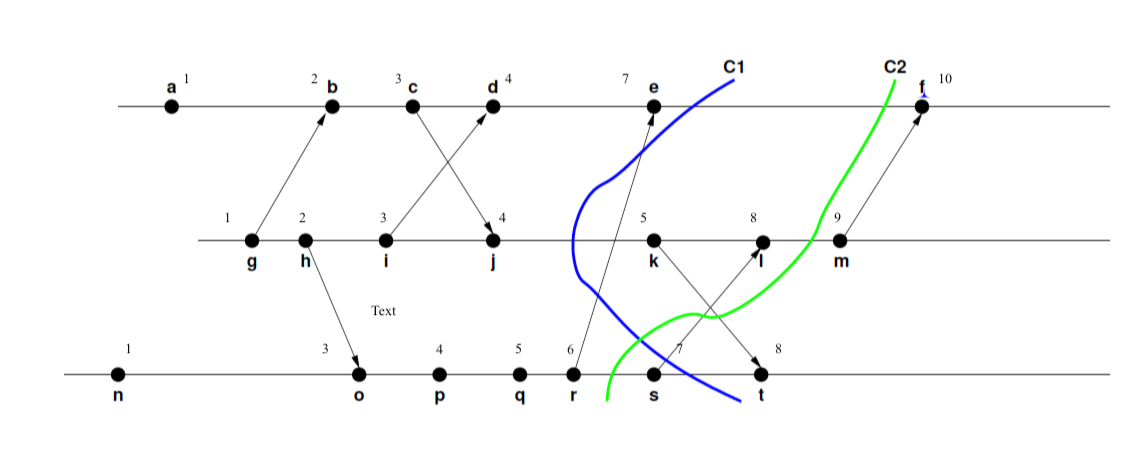
\includegraphics[width=6.5in]{LamportClock.png}\\
(b)\\
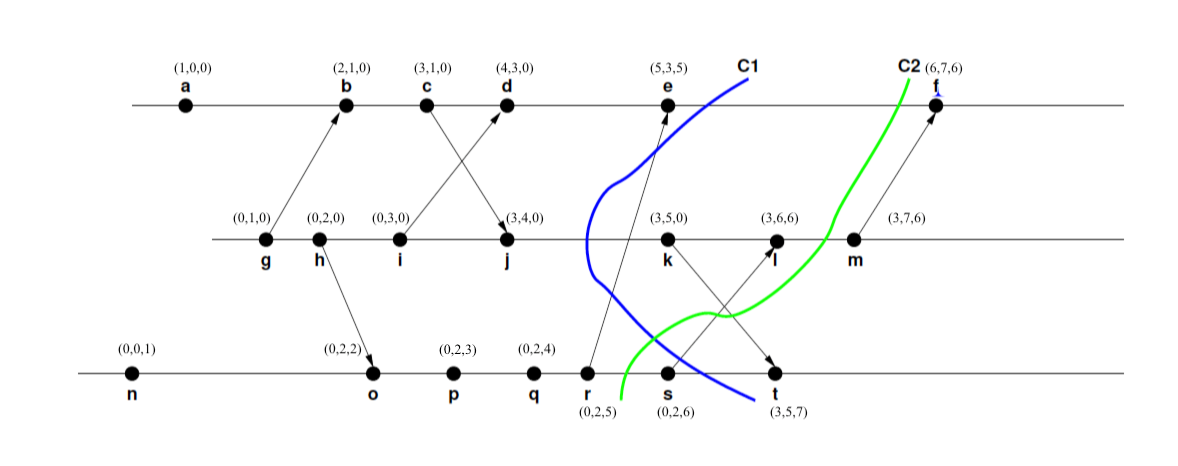
\includegraphics[width=6.5in]{VectorClock.png}\\
\newpage
(c)$C_1$ is consistent cut, $C_2$ is not consistent cut.\\\\
To be consistent cut, it must obey causality, if and only if for each pair of $e$, $f$, such that event $e$ is in the cut $C$, and if $f\prec e$, then event $f$ is also in the cut C.\\\\
For $C_1$, each pair of events are obeying this rule. To be noted, for event $s$, even though it was message sender in original system, it is acceptable that it is in the cut.\\\\
For $C_2$, one counter example is event $l$. It is a receiver event, which is in the cut. But its sender event $s$ is not in the cut, which results to be an Inconsistent Cut.\\
}

\problem{unisex bathroom problem using communicating sequential processes}{0}
\solution{
$UB = \mu X : \{malestudent,femalestudent\}\bullet(malestudent \to (malestudent \to (malestudent \to STOP))\ |\ femalestudent \to (femalestudent \to (femalestudent \to STOP)))$

}
\end{document}
